\section{Features explanation}
    In this thesis, the system must have the ability to control devices in the house in a convenient way, which means user can control devices from anywhere, anytime they want with an Internet-connected device and timer. Furthermore, the house should be capable of providing scenarios depends on the needs of user. For instance, users can switch on or off a number of specific devices by choosing a scenario instead of choosing individual device, namely “I’m home”, “Good night”, or “I’m leaving”. Based on the basic ideas, the thesis is integrated with all the basic features above. The thesis is designed for an one-floor house with three rooms, namely Living Room, Dining Room and Bedroom.
    \subsection{Convenient control}
    \subsubsection{Living Room}
    Front part of the house, which includes Main Door, Living Room and a Stair, the belonging AC devices will be controlled with four Relays but integrated into two Slave-Relay(s), one is Slave-3-Relays and the other is Slave-2-Relays (which is also integrated with the Relay controlling the Conditioner of Bedroom).
    \subsubsection{Dining Room}
    Second part of the house is assumed to have only one AC device and will be controlled with a Relay integrated on a Slave-2-Relays, in which has the Relay to control the Bedroom Light.
    \subsubsection{Bedroom}
    Last room of the house is Bedroom, in which is assumed to have two devices but one is integrated on the same circuit with Dining Room Light, the other is the Conditioner is also integrated on the same circuit with the Living Room Light.

    Apart from controlling the devices by physical Slave Button(s), which is also crossed implemented with no specific rule, the owner also can control the devices with a single Internet-connected device such as a smartphone, a tablet or a computer by accessing the Web Server from anywhere and anytime. Besides, it also has few scenarios that should be quite helpful for the owner. Imagine that when the owner arrive home after work, the devices needed are ready to serve such as the Front Light or the Conditioner. The project is also implemented with security camera block which helps user to access, monitor their house and receive alert in case of abnormal event happens in a convenient way with reasonable price. In addition, all data in the process of monitoring the house should be sent to a database, which helps the user and also engineer can keep track of the activities of devices in the house, then use the collected data to improve the experiences of the users in the future.

    \subsection{Block Diagram}

    \begin{figure}[!htp]
        \begin{center}
        \includegraphics[scale=0.55]{images/systemFullBlock.PNG}
        \caption{System Block Diagram}
        \label{fig:blockDiagram}
        \end{center}
    \end{figure}
    Figure~\ref{fig:blockDiagram} refers the overview of the system. From the block diagram, there are three main blocks, namely Master, Slaves and Internet Application block. In this thesis, each main block has different functions and may consists of one to many smaller blocks. Referring to Figure~\ref{fig:blockDiagram}, Master is in the middle, connects Slaves and Internet Application Block; Slaves are the “workers” depend on the Master and the Internet Block helps the User communicate with the system through Master remotely.
    \subsubsection{Master}
    As designed in section \ref{masterDesign}, Master is the circuit integrated with a STM32F4 Discovery Kit, connected via headers instead of being soldered directly on board in order to ensure an effortless replacement if broken. Beside the block of RS-485 module for main communication methodology and ESP-8266 for establishing connection to the Internet, it also has the headers for other modules of connectivity and functions in order to make the Master scalable in the future, namely SIM800A, Bluetooth module HC-05, and Real time module DS3231. However, instead of using an integrated Power block onto Master circuit, it uses a separated Power for Master as mentioned in section \ref{powerForMasterDesign}.

    Based on the basic idea, Master is responsible for receiving the requests from all sources, Slaves or Internet Application block, and distributing the command to the Slave with appropriate function. In addition, Master is also the middleman between Internet Application block with the Slaves, which means it also update the information between Internet application block and Slaves.
    \subsubsection{Slave Relay(s)}
    Slave Relay(s) (Slave \#1, \#2, \#3) consists of number of Relays (varies depends on users’ needs) and one PIC16F628A from Microchip as the MCU, responsible for switching AC devices On or Off based on the distributed command from Master.
    \subsubsection{Slave Button(s)}
    Slave Button(s) (Slave \#4-8) consists of number of Buttons (varies depends on users’ needs) and one PIC16F628A from Microchip as the MCU, responsible for controlling Slave Relay(s) by sending the commands to Master for the distribution to corresponding Slave Relay(s).
    \subsubsection{Internet Application Block}
    Internet Application block consists of smaller blocks with different functions, namely Database, Web Server, Internet connection block, Security Camera and Smart devices. Internet block establish the Internet connection for Master block; Web Server is the combination of back-end and front-end development of Webserver, besides helping users to control the system remotely with ease, the extended features will be explained later in this chapter; Security Camera responsible for recognizing person with Facial Recognition to open the door in order to cut off the steps of accessing the house. In addition, security camera is also integrated with motion detector prototype directly in Web Server. The Web Server communicates with the system through Internet block using MQTT protocol.

    \section{Communication Methodology and Algorithm of Master and Slaves}
    In this thesis, data is transmitted from UART of MCU to input of module RS-485 then to the data bus wire to distribute to corresponded components, noted that RS-485 is the physical standard which helps transmitted data travels much further compared to original UART. It needs two wires for data transmitting with module RS-485, but a cable of four wires is chosen for providing power supply of 12VDC and transmitting data at the same time with a single cable. Four wires in a cable with corresponded functions are listed as following.
    \begin{itemize}
    \item 12V: provide 12VDC throughout the system.
    \item A: Signal wire A.
    \item B: Signal wire B.
    \item GND: Common ground throughout the system.
    \end{itemize}

    However, RS-485 is a physical standard instead of an algorithm to distribute data through the whole network of a large number of devices with acceptable performance. Furthermore, in order for the chosen module RS-485 be able to work, its enable pin must be controlled by the MCU, which is set to logic 0 as default is receiving mode and vice versa. After sometimes reading books, the author suggested two algorithms for this thesis.
    \subsubsection{Ask/Request sequentially}
    \begin{itemize}
    \item \textbf{Master}: Master responsible for asking sequentially every connected Slaves in the system. After asking the Slaves for if they need to work, Master will delay for a small amount of time to wait for the response from Slaves. If the time is passed and asked Slave does not request to work, Master will pass that Slave and move on the next Slave. If a Slave Button is being asked but also receive the external signal, it can interrupt the process by sending a response to Master requesting to work, then that request will be prior to be sent to corresponded Slave Device. Now it ends the loop and start a new one. Period of time to ask the Slaves must be in milliseconds in order to complete the loop for every Slaves in the system.
    \item \textbf{Slave Button}: Slave Button has to wait for Master to ask and response. It is always stay in receiving mode (which has enable pin logic at 0 – LOW). When Slave Button is asked or an external signal comes in, it pulls enable pin to logic 1-HIGH to enter transmitting mode and response when Master asks.
    \item \textbf{Slave Device}: Enable pin of RS-485 of Slave Device is always in LOW status, which means receiving data mode. When Master ask or there is data transmitted from Slave Button, Slave Device will check if it is corresponded with its functions, if yes Slave Device will work as defined function.
    \end{itemize}
    
    With this algorithm, the asking loops will run continuously, and it should prevent two signal collide with one and another because the Slave only answers Master when Master asks. However, transmitted data will be difficult to be managed because of two reasons, waiting time and management. After a request is sent from Master, it takes some time for Master to wait for the response from Slave and pull enable pin of RS-485 to LOW. Besides, it takes times again to pull enable pin up to logic HIGH to distribute the response if available. This process is getting longer with the increment of the number of Slaves, which cause the transmission between Slaves become slower with a large number of Slaves. Furthermore, transmitting data continuously will consume loads of bandwidth leads to resource waste and cause errors dues to noise or inaccurate process from Slaves because of data is transmitted continuously leads to false data or worse is lose data. Thus, the author chose a different method to transmit data through the network based on CSMA/CD protocol.

\subsubsection{Work sequentially}
Based on the idea of CSMA/CD protocol, which is “Carrier-sense multiple access with collision detection”. It is explained briefly as if a node need to transmit data, it has to listen if the connection is busy or not. In the case the connection is idle, frame is transmitted, if not, that node has to wait a random time then start to listen again. In order to detect collision, transmitting node has to listen to the connection while transmitting data. If a collision is detected, that node has to stop transmitting and send a jam signal to others station while waiting a random time to start sending frame again.
In this thesis, the algorithm is built based on the working principle of CSMA/CD and Master-Slave model.
    \begin{itemize}
    \item \textbf{Master}: Master is the most important node in the network. After the system is booted up, Master will be ready and waiting for the transmission. The author could not complete the idea to set an identity for a new Slave entering the network, therefore, all identity will be pre-programmed and managed by the Master. Master now responsible as a middleman, receiving and distributing frames between Slaves in the network. Whenever a Slave Button send a frame to control assigned Slave Relay, Master will receive the frame then distributed to corresponding Slave Relay without a direct connection between any Slaves. With all the process, Master will pull up RS-485 to 1-HIGH when transmitting frame or pull down to 0-LOW (as default) when receiving frame.
    \item \textbf{Slave Button}: Slave Button will be in receiving mode (enable pin of RS-485 is 0-LOW) after booting up. When a button is pressed, it will pull up enable pin of RS-485 to 1-HIGH and send corresponding frame to Master for the distribution to the correct Slave Relay with corresponding identity. Then it returns to receiving mode to wait for the interruption again.
    \item \textbf{Slave Device}: Enable pin of RS-485 of Slave Device is always in LOW status, which means receiving data mode. When there is data transmitted from Slave Button, Slave Device will check if it is corresponded with its functions, if yes Slave Device will work as defined function.
    \end{itemize}

With this algorithm, Master will update Slave status after booting up, then Master and Slaves enter receiving mode to listen to transmission. It is an improvement in processing time and management compared to the previous algorithm. To be specific, frames are not transmitted relentlessly which saves large amount of resources and the delay is almost unnoticeable, this leads to the project can be extended to a number of slaves without much delays. Furthermore, the transmission is free in default, thus minimizes the chance that there will be two frame on the connection at the exact same time, this helps the frame is transmitted correctly with small probability that a collision is happened.

\subsection{Transmitting Frame Design}
    \subsubsection{Master to Slave Relays}
    In this thesis, a standard transmitting frame consists of 11 bytes as following.

    \begin{center}
    S$X_1$$X_2$$X_3$$X_4$$X_5$$X_6$$X_7$$X_8$$X_9$E
    \end{center}

    \textit{Explanation}:
    \begin{itemize}
        \item S: For recognition that a Frame is being transmitted.
        \item $X_1$: For recognition that the Master is transmitting to a Slave or vice versa. For instance, $X_1$=1 is Master transmits to Slave and $X_1$=0 is Slave transmits to Master.
        \item $X_2$: Byte for defined function. In this thesis, $X_2$=0 is the command controlling assigned Relay with a defined Button. $X_2$ has range from 0 to 9, which means the functions for the project can be extended up to 10 functions if necessary. 
        \item $X_3$$X_4$$X_5$: Bytes define identity of each component on Slave Relays or Slave Buttons. For instance, D01 is Relay number 1 (integrated on Slave-3-Relays in this thesis) or B02 is Button number 2 (integrated on Slave-3-Buttons in this thesis).
        \item $X_9$: Byte defines state of the device on Slave Relay which is being controlled. For instance, $X_9$=1 is “Turn device On” and $X_9$=0 is “Turn device Off”.
        \item $X_6$$X_7$$X_8$: Bytes that are reserved for further development.
        \end{itemize}

    \subsubsection{Slave Button to Master frames}
    Frame from Slave Buttons to Master is slightly different from frames from Master to Slave Relays.

        \begin{center}
        S$X_1$$X_2$$X_3$$X_4$$X_5$$X_6$$X_7$$X_8$$X_9$E
        \end{center}

    \textit{Explanation}:
    \begin{itemize}
    \item S: For recognition that a Frame is being transmitted.
    \item $X_1$: For recognition that the Master is transmitting to a Slave or vice versa. For instance, $X_1$=1 is Master transmits to Slave and $X_1$=0 is Slave transmits to Master.
    \item $X_2$: Byte for defined function. In this thesis, $X_2$=0 is the command controlling assigned Relay with a defined Button. $X_2$ has range from 0 to 9, which means the functions for the project can be extended up to 10 functions if necessary. 
    \item $X_3$$X_4$$X_5$: Bytes define identity of each Button on Slave Button. For instance, B01 is Button number 1 (integrated on Slave-3-Buttons in this thesis) or B04 is Button number 4 (integrated on Slave-2-Buttons in this thesis).
    \item $X_6$$X_7$$X_8$: Bytes define identity of each Relay on Slave Relays, which is the part to identify which Relay the Button needs to control. For instance, D01 is Relay number 1 (integrated on Slave-3-Relays in this thesis) or D02 is Relay number 2 (integrated on Slave-3-Relays in this thesis).
    \item $X_9$: Byte defines state of the device on Slave Relay which is being controlled. For instance, $X_9$=1 is “Turn device On” and $X_9$=0 is “Turn device Off”.
    \end{itemize}

    \begin{figure}[!h]
        \begin{center}
        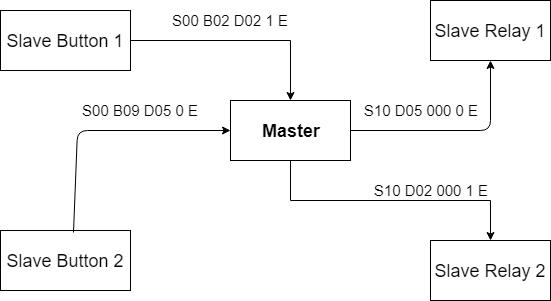
\includegraphics[scale=0.75]{images/frameEx.png}
        \caption{Example of transmitting frames}
        \label{fig:frameEx}
        \end{center}
    \end{figure}

    In particular, Figure~\ref{fig:frameEx} shows an example of frames transmitting in the system with the explanation above. The case of Slave Button 1 sends the frame of \textbf{S00 B02 D02 1 E} and Master sends a frame of \textbf{S10 D02 000 1 E} to Slave Relay 2 is explained in detail as following.
    \begin{itemize}
        \item S: For recognition that a Frame is being transmitted.
        \item $X_1$ = 0 indicates Slave Button 1 is sending to Master.
        \item $X_2$ = 0 indicates Slave Button 1 wants to control a Relay with the identity as of bytes $X_6$$X_7$$X_8$.
        \item $X_3$$X_4$$X_5$ = B02 indicates Button number 2 is controlling.
        \item $X_6$$X_7$$X_8$ = D02 indicates Button number 2 is controlling Relay number 2.
        \item $X_9$ = 1 is “Turn device On”.
    \end{itemize}

    \subsection{Working flowchart of Master and Slaves}
    In this section, the author shows the flowcharts of programs that are embedded in Master and Slaves. Each flowchart has a description below corresponding to its design. For instance, figure~\ref{fig:masterFlow}, figure~\ref{fig:buttonFlow} and figure~\ref{fig:relayFlow} indicates working principle of Master, Slave Button and Slave Relays, respectively.
    \begin{figure}[!htbp]
        \begin{center}
        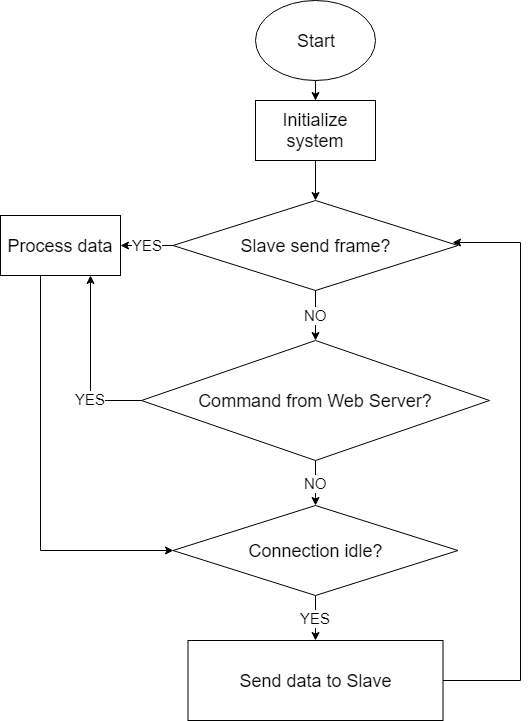
\includegraphics[scale=0.75]{images/masterFlow.png}
        \caption{Flowchart of Master}
        \label{fig:masterFlow}
        \end{center}
    \end{figure}
    \begin{figure}[!htb]
        \begin{center}
        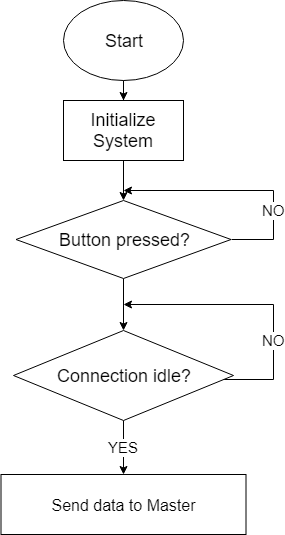
\includegraphics[scale=0.55]{images/buttonFlow.png}
        \caption{Flowchart of Slave Button}
        \label{fig:buttonFlow}
        \end{center}
    \end{figure}
    \begin{figure}[!htb]
        \begin{center}
        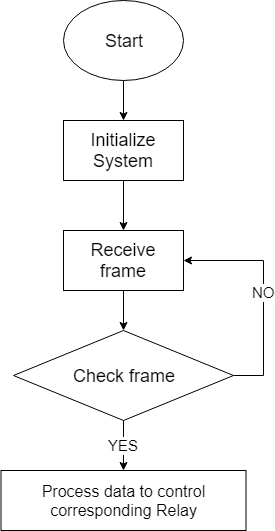
\includegraphics[scale=0.55]{images/relayFlow.png}
        \caption{Flowchart of Slave Relay}
        \label{fig:relayFlow}
        \end{center}
    \end{figure}

\newpage
\section{Internet Application Block Design}
Nowadays, Internet connection with its applications is the must have function for any smart system. This thesis is not fully implemented with Internet applications but the author chose the basic function that can support any user to live and control their house in an effortless way.
    \subsection{Internet Block} %esp8266
    In this thesis, Internet Block helps the user interact with the system through Wi-Fi connection with module NodeMCU ESP-8266. Beside establishing a connection between the Web Server and the system, it also handles the processing data phase in order to send a frame to Master.
        \subsubsection{MQTT Protocol}
        As for the connection between NodeMCU ESP-8266 and the Web Server, the author use MQTT protocol instead of HTTP. MQTT is an extremely lightweight protocol, designed for constrained devices. The topics for are designed with multiple levels to suits with the control methodology. For instance, NodeMCU is assigned as a client, which subscribes to the topic as shown in Figure~\ref{fig:espSub}.
        \begin{figure}[!htb]
            \begin{center}
            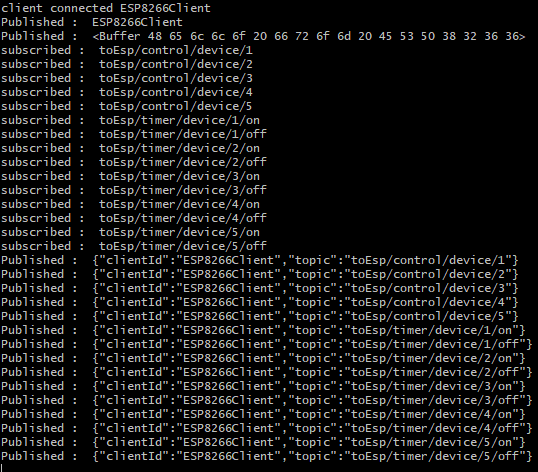
\includegraphics[scale=0.9]{images/espSub.png}
            \caption{Topics subscribed by NodeMCU}
            \label{fig:espSub}
            \end{center}
        \end{figure}

        \begin{figure}[!htbp]
            \begin{center}
            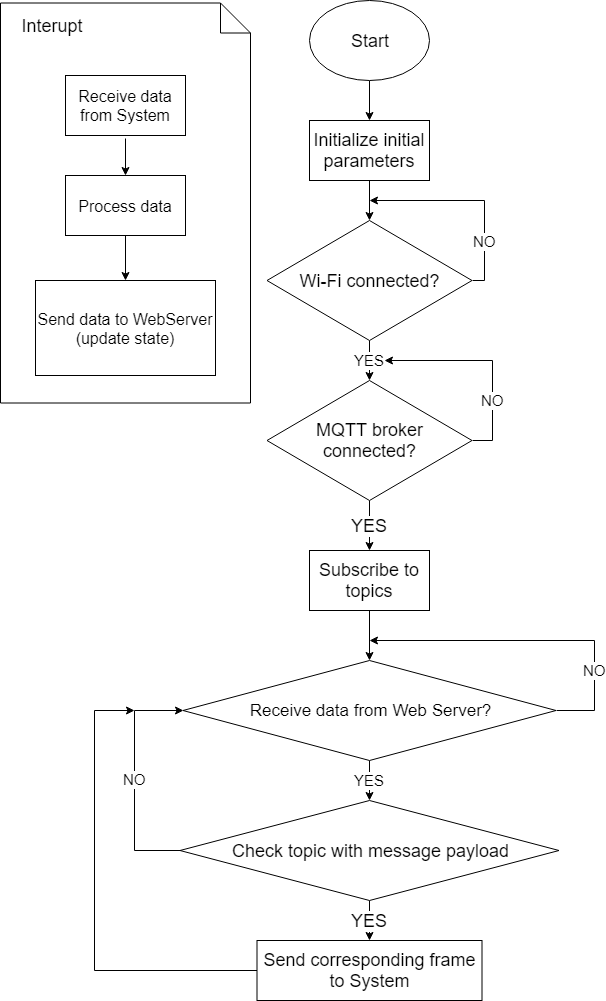
\includegraphics[scale=0.65]{images/mqttFlow.png}
            \caption{Flowchart of working principle of NodeMCU}
            \label{fig:mqttFlow}
            \end{center}
        \end{figure}
        In order to process the received data from Web Server, the author embedded a simple program for NodeMCU and Figure~\ref{fig:mqttFlow} illustrates its working principle.

    \subsection{Web Server}
    Web Server is the combination of Back-end and Front-end Design. To be specific, Back-end is the core for a Web Server which handles the logic and working flow of all components, Front-end is responsible for displaying the results of back-end processes and components to interacts. The author use Node.js for Back-end design and HTML, CSS for Front-end design.
        \subsubsection{Back-End Design}
        Node.js works on non-blocking I/O principle which makes it suitable for real-time applications included a real-time Web Server. Node.js empowers real-time web application by adopting push technology as against web sockets to build server-side web applications with two-way channel i.e. client and server. It operates on open web stack technologies like JavaScript, CSS, and HTML that work over the standard port 80. This tool is also lightweight both for in-memory usage and data dense real-time web applications that work on multiple devices. Figure~\ref{fig:nonBlocking} refers the working principle of Node.js in order to show its advantages for the Web Server in this Thesis.
        \begin{figure}[!htb]
            \begin{center}
            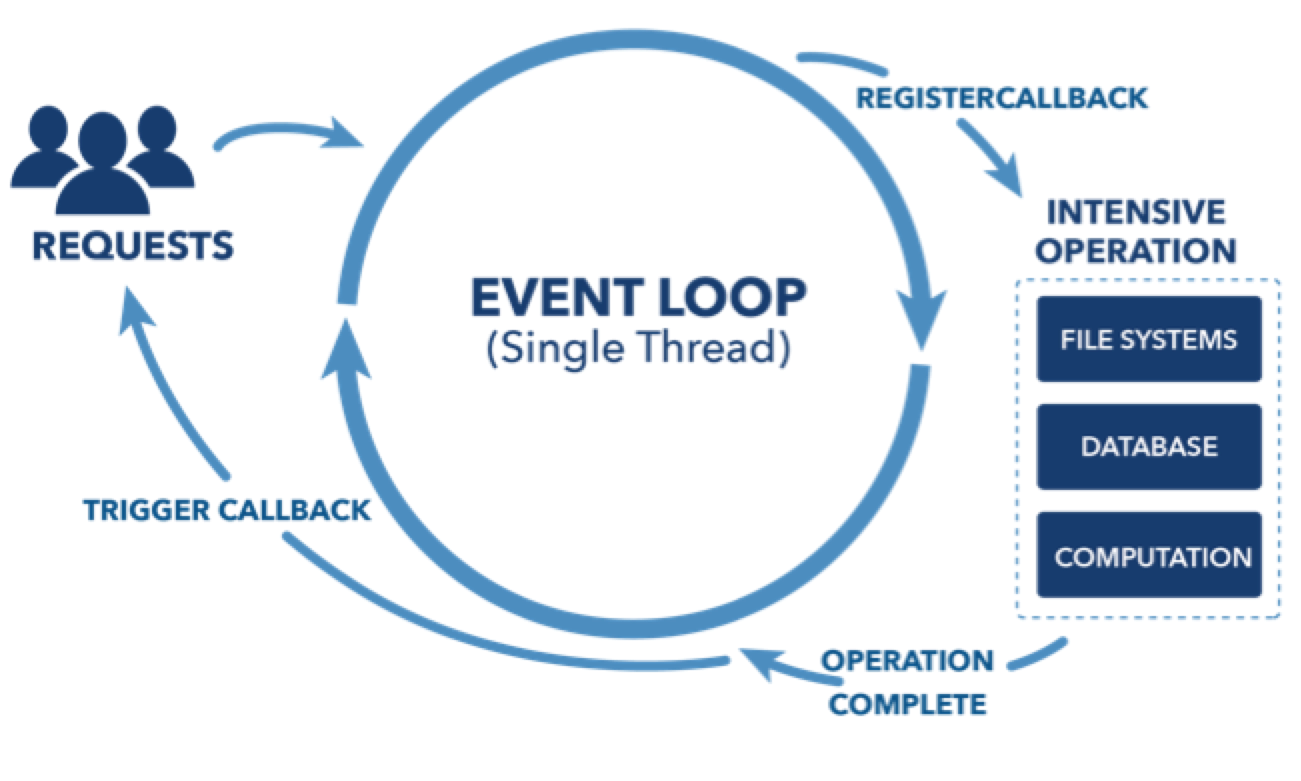
\includegraphics[scale=0.65]{images/nonBlocking.png}
            \caption{Node.js Working Principle}
            \label{fig:nonBlocking}
            \end{center}
        \end{figure}

        Server-side is implemented on port 2111 with MQTT protocol to communicate with other nodes in the network to control the system. In this thesis, the MQTT broker is running on port 3000 and written in Node.js using a module named Mosca, which makes a local and private Broker to implement MQTT protocol on. Figure~\ref{fig:webSub} shows the subscription of the Web Server to those topics which are in use of the Thesis.
        \begin{figure}[!htb]
            \begin{center}
            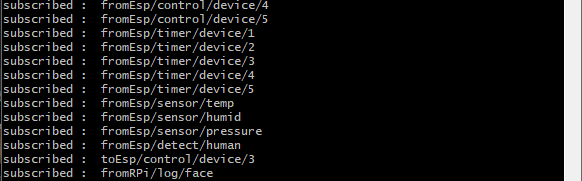
\includegraphics[scale=1]{images/webSub.png}
            \caption{Topics subscribed by Web Server}
            \label{fig:webSub}
            \end{center}
        \end{figure}

        In the Web Server, the author used both POST and GET methods in an appropriate way to ensure the sensitive information will not be exposed. For instance, the author used POST method for Log in information at Log in Page in order to make the information is not queried in the URL and GET method for getting page response to the Client.

        Because Web Server is an asynchronous application, it returns response to client whenever it receives a request from Client-side. After a successful log in session from the authorized person from the family, which means a default request is sent to Server-side to load the next page, Web Server is divided into four main pages corresponded to four function blocks, namely Dashboard, Control, Scenario and Indoor Security Camera. The activities of the devices will be logged into a Database, which helps to back up the data to monitor and should be used for future development. The figure~\ref{fig:responseBlock} illustrates the flowchart of every function blocks are implemented in this thesis that returns the corresponding response to Client-side.
        \begin{itemize}
            \item Dashboard: in this thesis, Dashboard page shows the overview of the system, namely the Sensor value (in the event a Slave Sensor is implemented) and Security Status of the Indoor Security Camera. Each component on this page will automatically retrieve the value from the Database, which is logged from the system in prior, and display for users with Front-end design.
            \item Control: Control page consists of the Button which help users to control devices on Slave Relay without pressing the physical buttons on Slave Buttons. This page is implemented with MQTT protocol to send command to the system and to receive state update from the system. Besides, a connection to the Database is also opened in order to log devices’ activities to monitor, maintain and develop in the future. The payload of the control message which is sent to corresponded topics is shown in the figure~\ref{fig:mqttPayload}. For instance, On is shown as “Buffer 6f 6e” and Off is “Buffer 6f 66 66”.
            \item Scenes: This page is implemented with four scenarios, namely Good Morning, I’m Home, Good Night and Security. The idea for this page is use the defined Scenarios to switch number of device On or Off in order to reduce the control time in similar circumstances. This page is also implemented with MQTT and a connection to Database to work as the same as Control Page.
            \item Indoor Security Camera: This page is a prototype implemented with Motion Detector using integrated WebCam of the computer. When the owner leaves the house, this function should be turned on and will be ready to detect the strange motion in an ideal condition that the house does not have any person or pet at home. If a motion is detected, it will send alert to the owner over Email and alert messages in all Pages if the Web Server is currently accessed by an authorized user, or in further development should be text messages over cellular network. It is also implemented with a connection to the Database to log the data in case of use in the future. The motion detection algorithm is done on Client-side, Server-side is responsible for receiving post-process data to raise alert in the event of strange motion occurs.
            \end{itemize}

        \begin{figure}[!htb]
            \begin{center}
            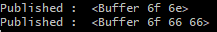
\includegraphics[scale=1.5]{images/mqttPayload.png}
            \caption{Control messages shown as Buffer Payload in corresponded topic}
            \label{fig:mqttPayload}
            \end{center}
        \end{figure}
        \begin{figure}[!htb]
            \begin{center}
            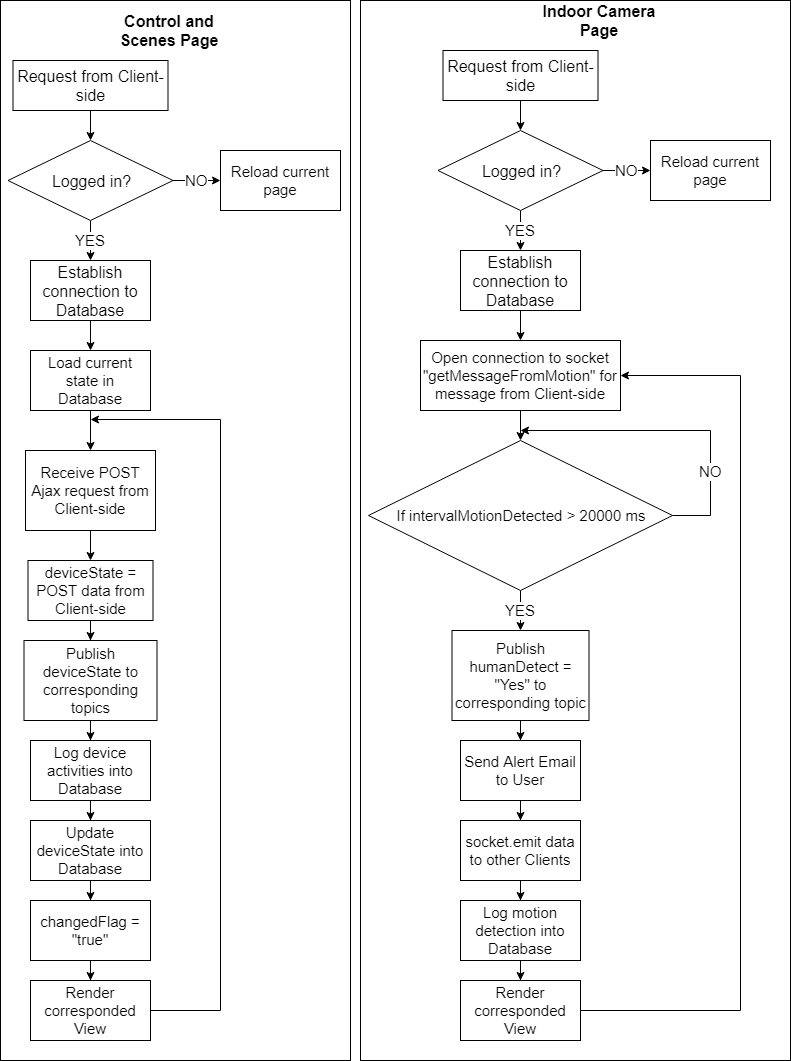
\includegraphics[scale=0.53]{images/responseBlock.png}
            \caption{Flowchart of each function blocks in Web Server}
            \label{fig:responseBlock}
            \end{center}
        \end{figure}

        \newpage
        \subsubsection{Front-End Design}
        Front-end design is the combination of languages, namely Javascript, HTML5 and CSS. With Node.js, the author is able to write both back-end and front-end in Javascript, which helps reduce plenty of time. Front-end design particularly means design the \gls{hmi} and the communication between Client-side and Server-side with Ajax technique, tools and libraries, namely jQuery, Bootstrap or Socket.io, which should help end-user interact with the application in an effortless way. The result of HMI will be shown in Chapter \ref{result}. Besides, Motion detection algorithm is shown as in figure~\ref{fig:motionFlow} and it is done in Client-side.
        \begin{figure}[!h]
            \begin{center}
            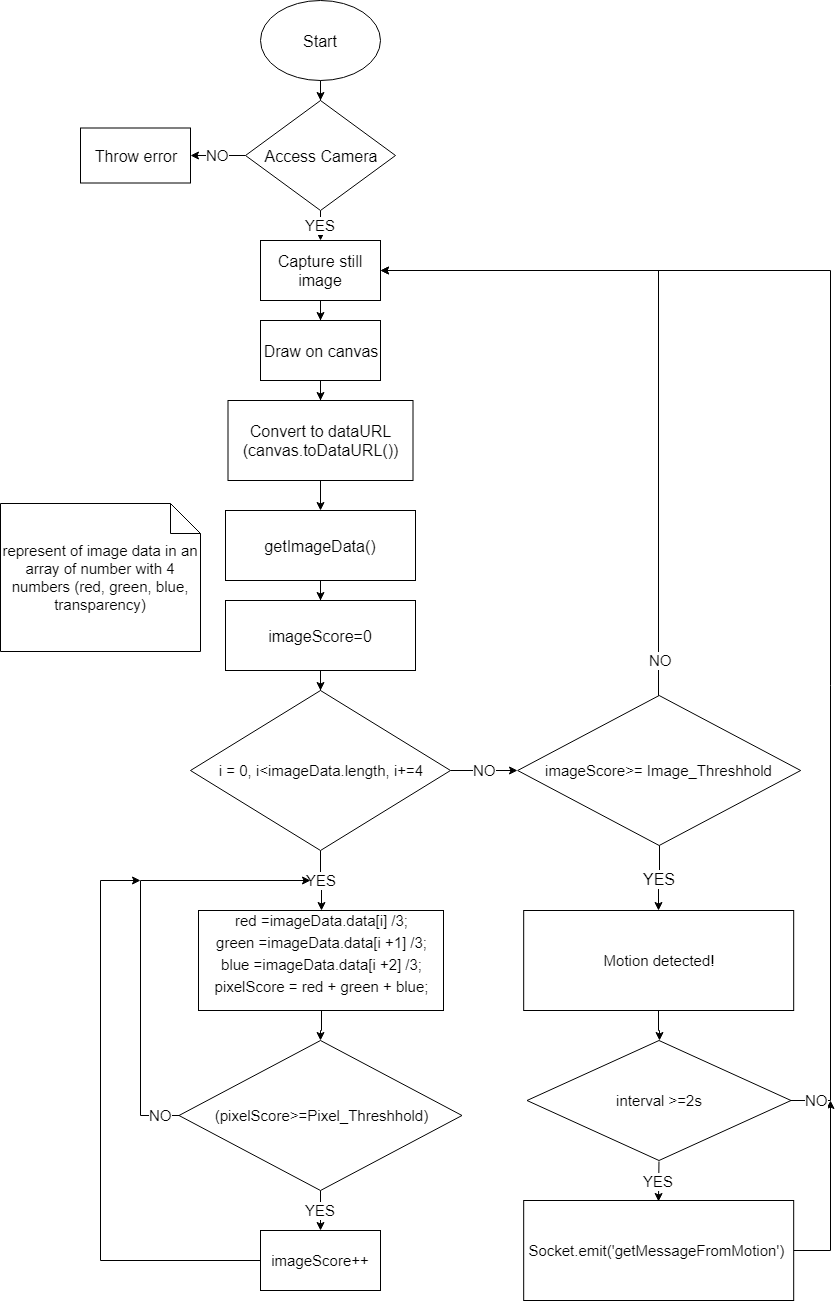
\includegraphics[scale=0.45]{images/motionFlow.png}
            \caption{Flowchart of Indoor Security Camera}
            \label{fig:motionFlow}
            \end{center}
        \end{figure}

    \subsection{Database}
    Database is a collection of data, create and managed in relational or non-relational way. In this thesis, the author chose MongoDB, a non-relational database. The database works similar to an electronic warehouse where data is organized and kept in categories and value by using key/value pair. To be specific, MongoDB stores data in BSON file, which is similar to JSON format, therefore easy to manipulate the stored data.

    In this thesis, the author organizes data with four collections, namely floor1, logDeviceActivities, logFaceDetection and logMotion. Each collection responsible for logging corresponding data. To be specific, floor1 stores all devices in houses with their id, name and state. In addition, logDeviceActivities, logFaceDetection and logMotion have timestamp in details to identify the time of any interaction with the house and its devices. Furthermore, logDeviceActivities and logFaceDetection also show deviceId with its State and person who accessed with the permission at the same time, respectively. Please see the figure~\ref{fig:floor1}, figure~\ref{fig:logDevice}, figure~\ref{fig:logFace} and figure~\ref{fig:logMotion} for the key/value pair of each collections.
    \begin{figure}[!ht]
        \begin{center}
        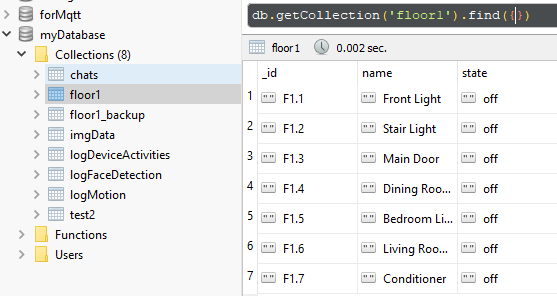
\includegraphics[scale=0.8]{images/floor1.png}
        \caption{Data of collection Floor1}
        \label{fig:floor1}
        \end{center}
    \end{figure}
    \begin{figure}[!ht]
        \begin{center}
        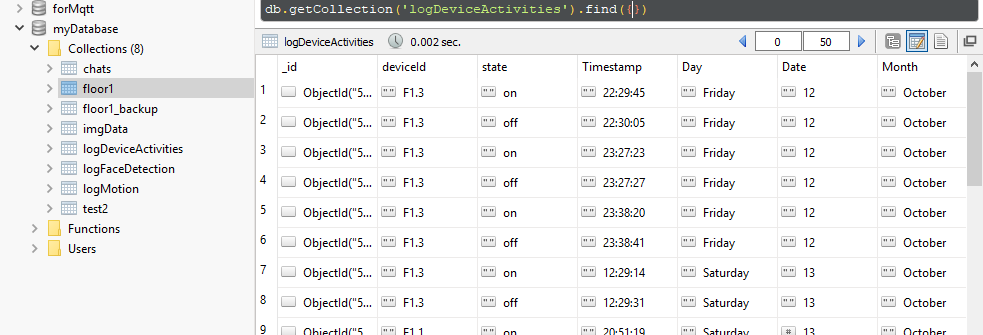
\includegraphics[scale=0.55]{images/logDevice.png}
        \caption{Data of collection logDeviceActivities}
        \label{fig:logDevice}
        \end{center}
    \end{figure}
    \begin{figure}[!ht]
        \begin{center}
        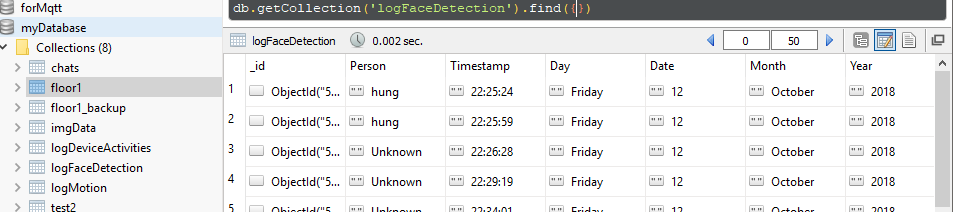
\includegraphics[scale=0.55]{images/logFace.png}
        \caption{Data of collection logFaceDetection}
        \label{fig:logFace}
        \end{center}
    \end{figure}
    \begin{figure}[!ht]
        \begin{center}
        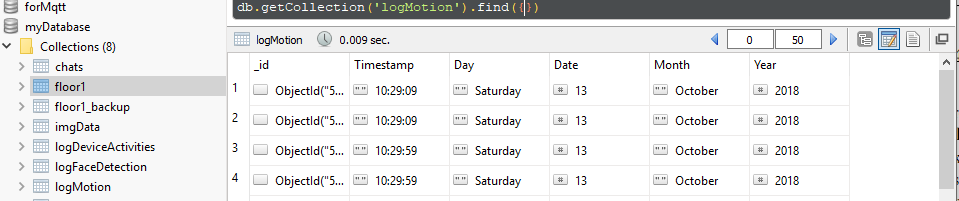
\includegraphics[scale=0.55]{images/logMotion.png}
        \caption{Data of collection logMotion}
        \label{fig:logMotion}
        \end{center}
    \end{figure}
 
    \subsection{Security Camera Block}
    Security Camera Block is implemented in the minicomputer named Raspberry Pi 3 Model B. The programme is written in python and implemented with OpenCV for Facial Recognition, in which OpenCV is a library aimed at real-time computer vision projects. Raspberry Pi 3 is installed with Raspbian OS and attached PiCamera Module via CSI port. With the help of OpenCV, the author is able to implemented a real-time facial recognition system with acceptable results. Because it is implemented in Raspberry Pi, the security camera block is capable of running full time when setup at front door with a power supply and a small monitor. Because the author is limited in resource, the Raspberry Pi screen will be displayed directly on laptop with a software for demonstration.

    The programme running on Raspberry Pi is designed with a simple HMI, in which user can interact by virtual buttons on it. The functions of each button is described as following.
    \begin{itemize}
        \item Start Face Recognition: Run Facial Recognition, if recognized, the Main Door is automatically open by publishing a message to topic \textit{toEsp/control/device/3} of MQTT protocol. The data to be published is the returned value of \textit{global\_id} as refers in last step of Recognition step from Figure~\ref{fig:recognize}.
        \item Close Door: After the Door is opened, user can close the it on the screen with this virtual Button, without using a physical button or the Web Server.
        \item RESTART: restart the software in Raspberry Pi if needed without using lines of command, which suits for an user.
        \item Log in as ADMIN!: is used to log into the system with the correct password. This button is useful when the user wants to add more data of allowed people into the dataset. After logged in, a simple UI of Register function appears with two steps of “Register” and “Train data” as following  to prepare for the Facial Recognition in the main UI, which will be explained explicitly in the same section.
            \begin{itemize}
            \item Register: is data gathering step which capture and save the images into local storage, downscale and transform to lighten the load and reduce the processing time. Figure~\ref{fig:dataset} illustrates the working flow of Register function, which is used to gather data to train in next step. The parameters are mentioned in the aside notes in the flowchart has description as following. Gray is the input grayscale images in previous step, scaleFactor specifies how much the image should be reduced in size and minNeighboors is specifies how many neighbors each candidate rectangle should have, to retain it. A higher number gives lower false positives.
            \item Train data: the step to feed the newly added faces from previous step for the face recognizer to train using LBPH algorithm, which is already built in OpenCV. Figure~\ref{fig:train} illustrates the training step of the recognizer.
            \end{itemize}
        \end{itemize}
        \begin{figure}[!ht]
            \begin{center}
            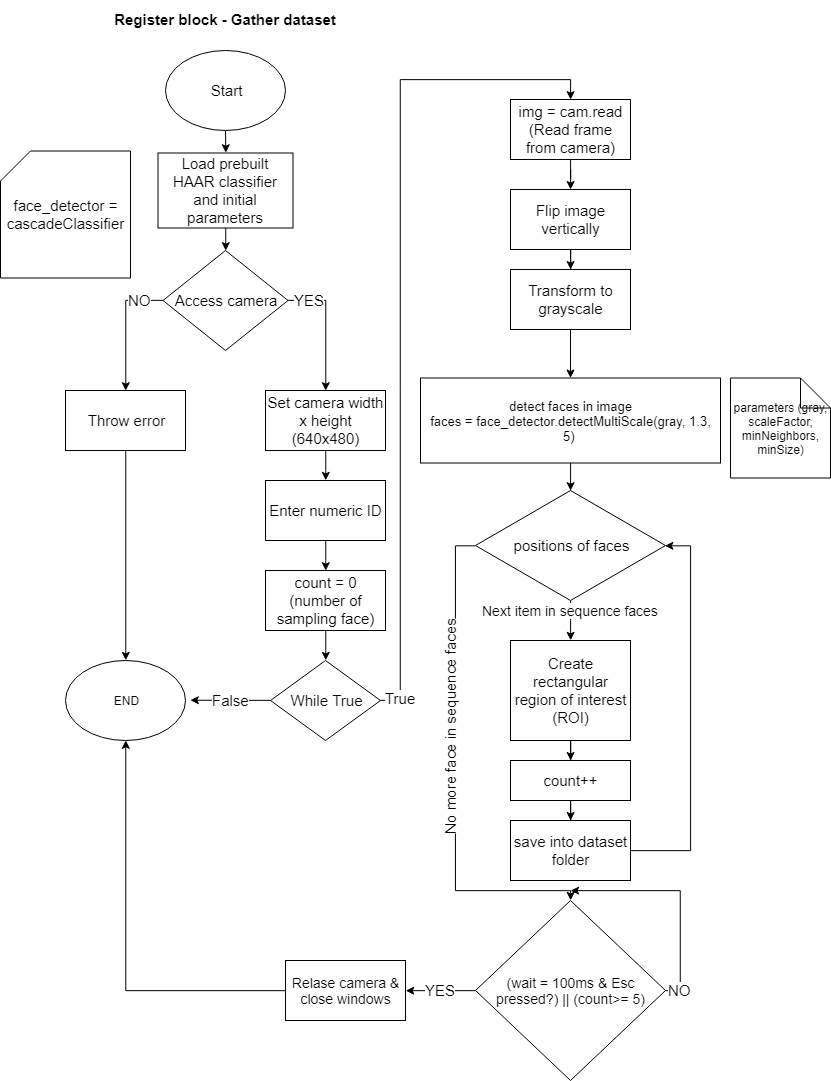
\includegraphics[scale=0.5]{images/dataset.png}
            \caption{Flowchart of Register step - Gathering dataset}
            \label{fig:dataset}
            \end{center}
        \end{figure}
        \begin{figure}[!ht]
            \begin{center}
            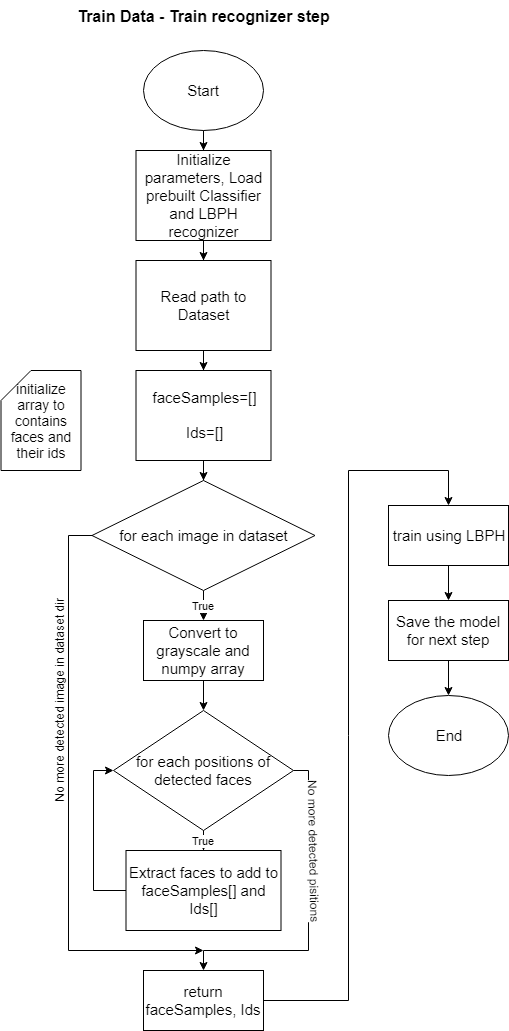
\includegraphics[scale=0.64]{images/train.png}
            \caption{Flowchart of Train data step - Training from dataset}
            \label{fig:train}
            \end{center}
        \end{figure}
        \begin{figure}[!ht]
            \begin{center}
            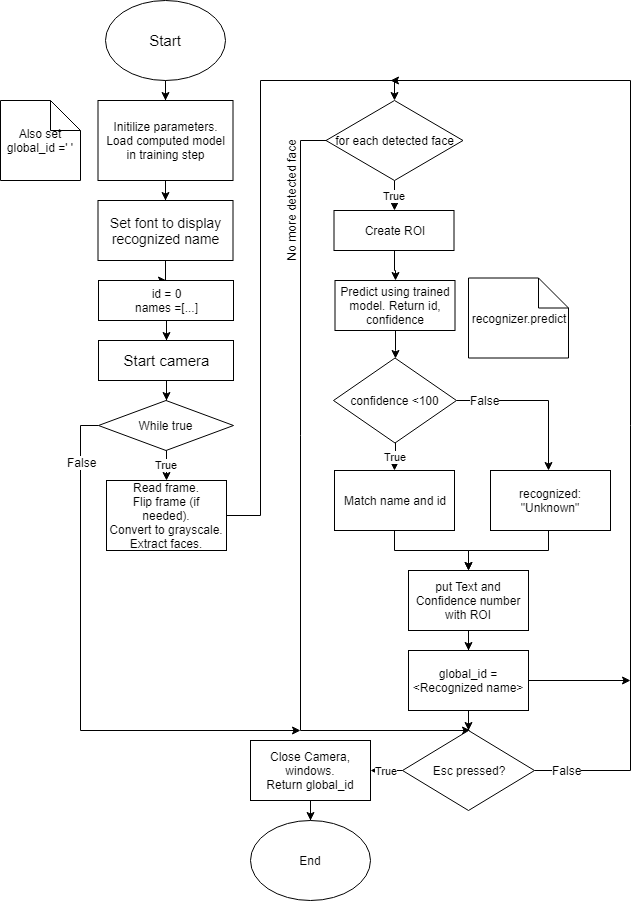
\includegraphics[scale=0.65]{images/recognize.png}
            \caption{Flowchart of Recognition step - Recognition from trained data}
            \label{fig:recognize}
            \end{center}
        \end{figure}
        
        
        
    


        





